% STEP 1: Choose oneside or twoside. Use the 'draft' option a lot when writing.
\documentclass[english, oneside]{HYgradu}

\usepackage[utf8]{inputenc} % For UTF8 support. Use UTF8 when saving your file.
\usepackage{lmodern} % Font package
\usepackage{textcomp}
\usepackage[pdftex]{color, graphicx} % For pdf output and jpg/png graphics
\usepackage[pdftex, plainpages=false]{hyperref} % For hyperlinks and pdf metadata
\usepackage{fancyhdr} % For nicer page headers
%\usepackage{tikz} % For making vector graphics (hard to learn but powerful)
%\usepackage{wrapfig} % For nice text-wrapping figures (use at own discretion)
\usepackage{amsmath, amssymb} % For better math
\usepackage[round]{natbib} % For bibliography
\usepackage[footnotesize,bf]{caption} % For more control over figure captions
\usepackage{subcaption}

\fussy % Probably not needed but you never know...


% OPTIONAL STEP: Set up properties and metadata for the pdf file that pdfLaTeX makes.
% But you don't really need to do this unless you want to.
\hypersetup{
    bookmarks=true,         % show bookmarks bar first?
    unicode=true,           % to show non-Latin characters in Acrobat’s bookmarks
    pdftoolbar=true,        % show Acrobat’s toolbar?
    pdfmenubar=true,        % show Acrobat’s menu?
    pdffitwindow=false,     % window fit to page when opened
    pdfstartview={FitH},    % fits the width of the page to the window
    pdftitle={},            % title
    pdfauthor={},           % author
    pdfsubject={},          % subject of the document
    pdfcreator={},          % creator of the document
    pdfproducer={pdfLaTeX}, % producer of the document
    pdfkeywords={something} {something else}, % list of keywords for
    pdfnewwindow=true,      % links in new window
    colorlinks=true,        % false: boxed links; true: colored links
    linkcolor=black,        % color of internal links
    citecolor=black,        % color of links to bibliography
    filecolor=magenta,      % color of file links
    urlcolor=cyan           % color of external links
}

% STEP 2:
% Set up all the information for the title page and the abstract form.
% Replace parameters with your information.
\title{Formation of cores by merging supermassive black holes}
\author{Joonas Suortti}
\date{\today}
\level{Master's thesis}
\faculty{Faculty of Whatever}
\department{Department of Something}
\address{PL 42 (Kuvitteellinen katu 1)\\00014 Helsingin yliopisto}
\subject{Your Field}
\prof{prof. Smith}
\censors{prof. Smith}{doc. Smythe}{}
\depositeplace{}
\additionalinformation{}
\numberofpagesinformation{\numberofpages\ pages}
\classification{}
\keywords{Your keywords here}
\quoting{``Bachelor's degrees make pretty good placemats if you get them laminated.'' \\---Jeph Jacques}

\begin{document}

% Generate title page.
\maketitle

% STEP 3:
% Write your abstract (of course you really do this last).
% You can make several abstract pages (if you want it in different languages),
% but you should also then redefine some of the above parameters in the proper
% language as well, in between the abstract definitions.
\begin{abstract}
Abstract goes here.
\end{abstract}

% Place ToC
\mytableofcontents



% -----------------------------------------------------------------------------------
% STEP 4: Write the thesis.
% Your actual text starts here. You shouldn't mess with the code above the line except
% to change the parameters. Removing the abstract and ToC commands will mess up stuff.
\chapter{Introduction}

\chapter{Theory}

\chapter{KETJU}

\chapter{Merger Simulations Using KETJU}

We analyse the results of two simulation sets of galaxy mergers with central supermassive black holes, both done using the KETJU code by \cite{Mannerkoski2019} and \cite{Rantala2018}. This is done in order to determine if merging SMBHs are able to cause the formation of cored galaxies, how the black hole masses affect the size of the core, and if the KETJU-code produces merger remnants comparable to observations. 

\section{Simulation Details}

All of the different simulation runs analysed, use merger progenitor galaxies from the same progenitor pool. There are seven different progenitors in total. Six of them (BH-1 - BH-6) contain central supermassive black holes, with the BH masses varying from $8.5 \times 10^8 M_\odot$ to $8.5 \times 10^9 M_\odot$. The seventh progenitor (BH-0) doesn't have an SMBH in its centre, and is included for the sake of comparison. The detailed masses of the progenitors' central SMBHs are listed in table \ref{table:progenitors}. Apart from the SMBH masses however, all of the progenitor galaxies have identical physical properties. These properties are described in table \ref{table:properties}, while the reasoning behind them is explained in \cite{Rantala2018} (do I have to go into same amount of detail as in the paper?).

Alongside the physical properties, the distributions of the different particles that make up the progenitor galaxies are also identical. Not counting the central point mass SMBH, all of the particles are distributed according to a Dehnen density-potential model \citep{Dehnen1993}:
\begin{equation}
\rho(r) = \frac{(3-\gamma)M}{4\pi} \frac{a}{r^\gamma (r+a)^{4-\gamma}},
\end{equation}
\begin{equation}
\phi(r) = \frac{GM}{a} \times 
\begin{cases}
	-\frac{1}{2-\gamma} \left[ 1 - \left( \frac{r}{r+a} \right)^{2-\gamma} \right] & \; \gamma \neq 2 \\
	\ln \frac{r}{r+a}	 & \; \gamma = 2
\end{cases},
\end{equation}
where $M$ is the total mass, $a$ is a scaling radius, and $\gamma$ is the central slope of the profile. The fundamental difference between the models describing the distribution of the rest of the particles, i.e. stellar and dark matter particles, is that for stellar particles the value used for $\gamma$  is $3/2$, while for the dark matter particles $\gamma = 1$.

\begin{table}
	\begin{center}
		\begin{tabular}{c c}
		\hline
		\hline
		Progenitor & $M_\bullet$ [$\times 10^9 M_\odot$] \\
		\hline
		BH-0 & - \\
		BH-1 & $0.85$ \\
		BH-2 & $1.7$ \\
		BH-3 & $3.4$ \\
		BH-4 & $5.1$ \\
		BH-5 & $6.8$ \\
		BH-6 & $8.5$ \\
		\hline
		\end{tabular}
	\end{center}
	\caption{Central SMBH masses of the progenitors used in the analysed simulations.}
	\label{table:progenitors}
\end{table}

\begin{table}
	\begin{center}
		\begin{tabular}{c c c c c c}
		\hline
		\hline
		$M_\star$ & $R_e$ & $M_\mathrm{DM}$ & $f_\mathrm{DM}(r_{1/2})$ & $N_\star$ & $N_\mathrm{DM}$ \\
		$[\times 10^{11} M_\odot]$ & $[\mathrm{kpc}]$ & $[\times 10^{13} M_\odot]$ & & & \\
		\hline
		$4.15$ & $7$ & $7.5$ & $0.25$ & $4.15 \times 10^6$ & $1.0 \times 10^7$ \\
		\hline
		\end{tabular}
	\end{center}
	\caption{The physical properties, constant throughout the different progenitor galaxies: \\
	$M_\star$: Stellar mass \\
	$R_e$: Effective radius \\
	$M_\mathrm{DM}$: Mass of the dark matter halo \\
	$f_\mathrm{DM}(r_{1/2})$: Fraction of dark matter mass compared to stellar mass inside the effective radius \\
	$N_\star$: Number of stellar particles \\
	$N_\mathrm{DM}$: Number of dark matter particles}
	\label{table:properties}
\end{table}

While the merger progenitor galaxies are the same, the initial conditions of the simulations are quite different. The \cite{Mannerkoski2019} simulations comprise of four subsequent runs, where, initially the progenitor galaxy BH-6 (table \ref{table:progenitors}), and later the remnant of the previous merger, is merged with the progenitor BH-2. On the other hand, the simulations done by \cite{Rantala2018} contain simply seven different mergers between two of the same progenitor galaxies.

The results gathered from the two sets of simulations also differ from each other. From the simulations done by \cite{Mannerkoski2019}; the locations, velocities and masses of the central SMBHs are saved. The data comes from time steps starting from when the semi-major-axis of the merging SMBH binary is $a \lesssim 5000 R_s$ ($R_s$ is the Schwarzschild radius) up until the end of the simulation. The simulation results of \cite{Rantala2018}, however, consists of not only the properties of the black holes, but also the stellar particles and dark matter particles, in the form of a single snapshot at the simulation time $t = 2 \mathrm{Gyr}$. Due to the distinct difference between the type of results gained from the two different simulation sets (and for simplicity's sake), we will from now on be calling the simulations from \cite{Mannerkoski2019} "Runs", and the ones from \cite{Rantala2018} "Snapshots" (table \ref{table:runs_and_snaps}).

\begin{table}
	\begin{center}
		\begin{tabular}{| c | c c | c | c c |}
		\hline
		\multicolumn{3}{|c|}{\cite{Mannerkoski2019}} & \multicolumn{3}{|c|}{\cite{Rantala2018}} \\
		\hline
		Run & $M_{\bullet, 1} [10^9 M_\odot]$ & $M_{\bullet, 2} [10^9 M_\odot]$ & Snapshot & $M_{\bullet, 1} [10^9 M_\odot]$ & $M_{\bullet, 2} [10^9 M_\odot]$ \\
		\hline
		1 & $8.5$ & $1.7$ & 0 & - & - \\
		2 & $10.2$ & $1.7$ & 1 & $0.85$ & $0.85$ \\
		3 & $11.9$ & $1.7$ & 2 & $1.7$ & $1.7$ \\
		4 & $13.6$ & $1.7$ & 3 & $3.4$ & $3.4$ \\
		 &  &  & 4 & $5.1$ & $5.1$ \\
		 &  &  & 5 & $6.8$ & $6.8$ \\
		 &  &  & 6 & $8.5$ & $8.5$ \\
		\hline
		\end{tabular}
	\end{center}
	\caption{Central SMBH masses of the progenitors used in the different simulation runs.}
	\label{table:runs_and_snaps}
\end{table}

\section{Black Hole Trajectories}

\begin{figure}[h]
	\centering	
	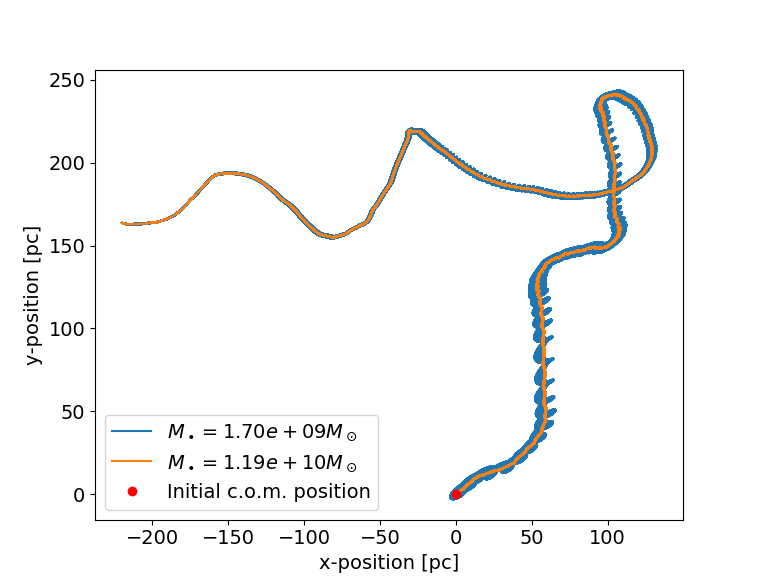
\includegraphics[width=0.7\textwidth]{Run3_Trajectory.png}	
	\caption{The trajectories of the black holes during "run 3" of the simulation. The coordinates are centred on the initial location of the centre-of-mass of the black hole system. The orange and blue lines show the paths taken by the smaller and larger black holes respectively during the simulation. Both paths show clear spiral patterns which become smaller and smaller as the simulation proceeds. The paths end at the location where the black holes merge, i.e. where the distance between them is below the specific threshold.}
\end{figure}

\begin{figure}[h]
	\centering
	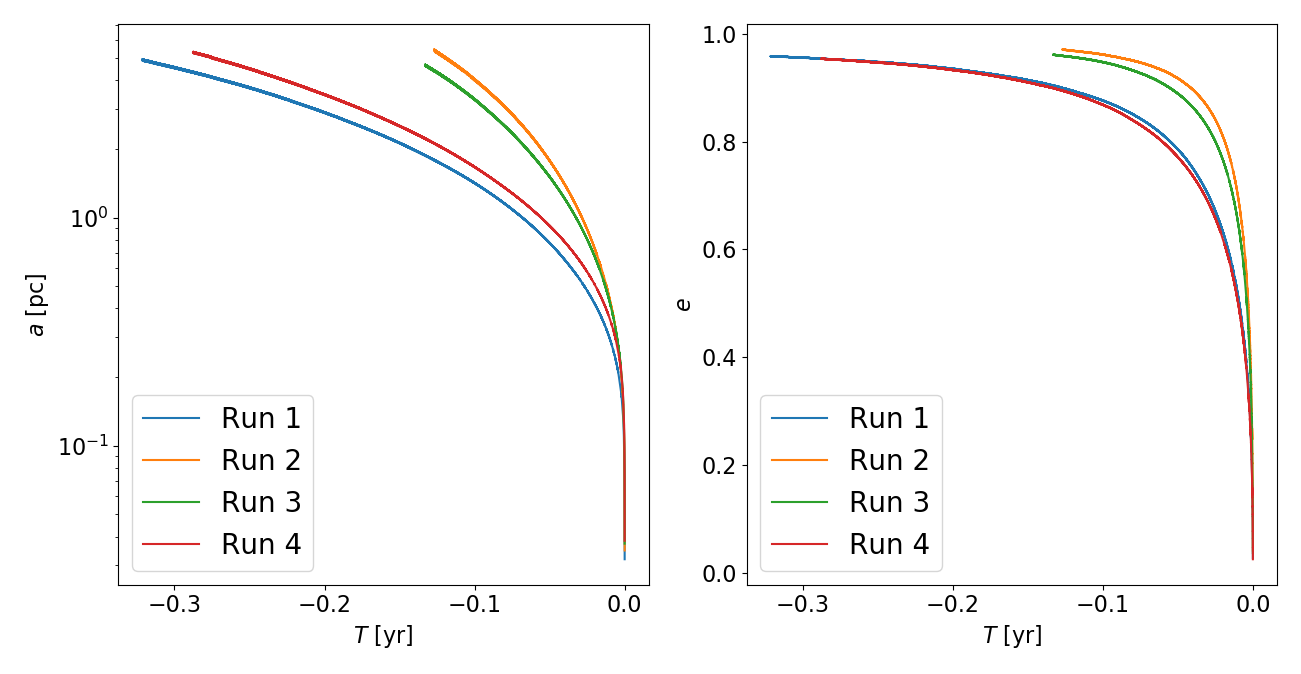
\includegraphics[width=\textwidth]{semi_major_and_ecc.png}
	\caption{The semi-major axes (left) and eccentricities (right) of the black hole systems in simulation runs 1-4 as a function of time. The zero position on the x-axis corresponds to the point of time in the simulation, where the black hole merging event happens.}
\end{figure}

\section{Core Size Measurements}

In order to check if a merger remnant is cored or not, we first have to calculate their surface brightness profiles. As the "Runs" don't contain stellar data, we use the "Snapshots" for the core analysis. 

We calculate the surface brightness profiles from the snapshots by: changing the coordinate system to centre-of-mass coordinates, projecting the stellar particles onto a plane, and calculating masses inside logarithmically space radial bins to get a radial mass surface density profile. We then do the aforementioned calculations 100 times from random viewing angles and calculate the azimuthal average of the profiles. This allows us to form a smooth mass surface density profile, which we then turn into a surface brightness profile by assuming a mass-to-light ratio of $M/L = 4$ \citep{Rantala2018}. In figure \ref{figure:surface_brightness}, one can see example surface brightness profiles for all of the snapshots. Looking at the different curves, it seems like the presence of central SMBHs in the progenitor galaxies does cause some kind of brightness deficiency near the galactic centre of the remnant's surface brightness profile. Not only that, the higher the mass of the central black holes in the progenitor galaxies, the larger the surface brightness deficiency seems to be.

\begin{figure}[h]
	\centering
	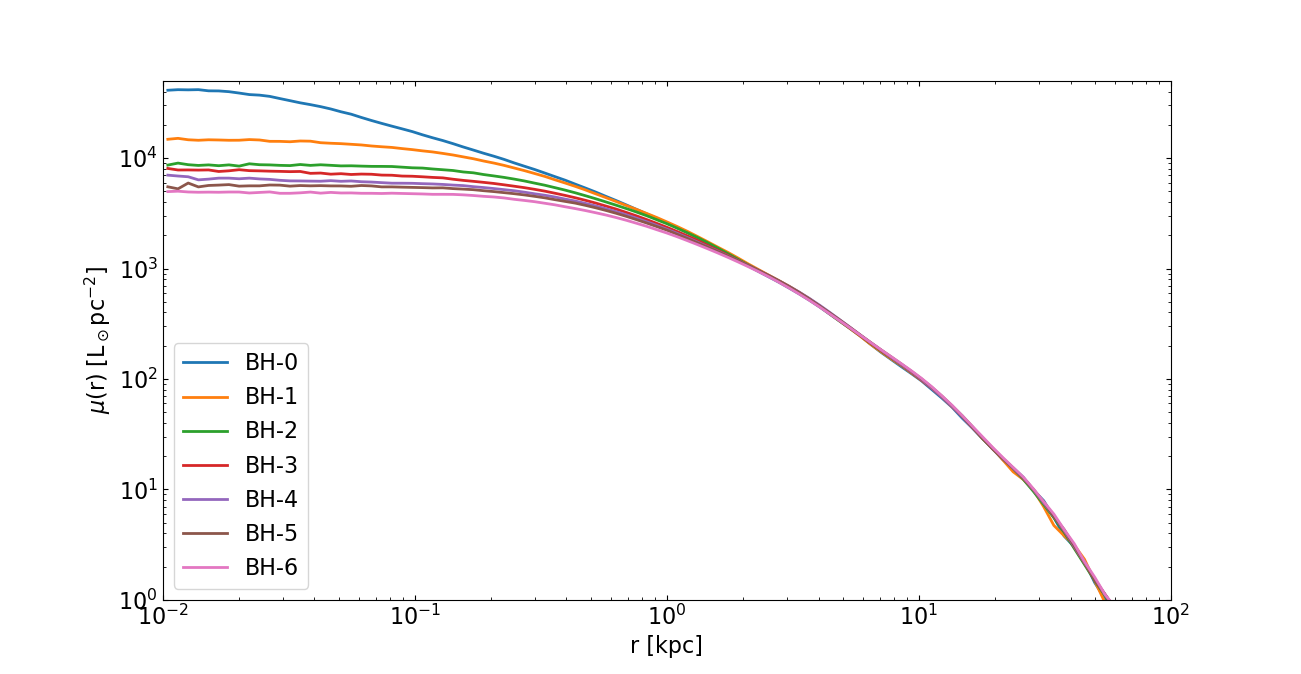
\includegraphics[width=\textwidth]{SurfaceBrightnessProfiles.png}
	\caption{Surface brightness profiles of all of the simulated merger remnants. The profiles were calculated by dividing the remnants into 100 radial bins, and averaging the surface brightness inside the bins through 100 random viewing angles. The luminosity of the particles was estimated by assuming a mass-to-light ratio of $M/L = 4$.}
	\label{figure:surface_brightness}
\end{figure}

The surface brightness profiles mentioned above do seem to indicate the presence of cores in the merger remnants with merging SMBH binaries. Determining the precise size of the core requires us to find the exact location where the deviations from the expected power-law profile start. This can be done by fitting the calculated profile with a model that is a combination of two power laws, a shallow inner power-law and steeper outer power-law. The location where the power laws change, i.e. the break radius $r_b$ is equivalent to the radius of the core. 

There are two commonly used options for modelling the surface brightnes profiles. The first one is the core-Sérsic profile \citep{Graham2003}, which can be expressed using the following equation:
\begin{equation}
\mu(r) = \mu' \left[ 1 + \left( \frac{r_b}{r} \right)^\alpha \right]^{\gamma / \alpha} \exp \left\lbrace -b_n \left[ \left( r^\alpha + r_b^\alpha \right) / r_e^\alpha \right]^{1/(\alpha n)} \right\rbrace, \label{eq:core-sersic}
\end{equation}
where $r_b$ is the break radius (i.e. the core radius), $\gamma$ is the logarithmic slope of the inner power-law, $\alpha$ controls the sharpness of the transition between the two power-laws, $r_e$ and $n$ are the effective half-mass radius and the Sérsic index of the outer power-law, and the normalization factor $\mu'$ is defined by:
\begin{equation}
\mu' = \mu_b 2^{-\gamma/\alpha} \exp \left[ b_n \left( 2^(1/\alpha) r_b/r_e \right)^{1/n} \right], 
\label{eq:mu_dot}
\end{equation}
where $\mu_b$ is the surface brightness at the break radius. 

The second option for determining the core radius through profile fitting, is using the so called Nuker profile \citep{Lauer1995}:
\begin{equation}
\mu(r) = 2^{(\beta - \gamma) / \alpha} \mu_b \left( \frac{r_b}{r} \right)^\gamma \left[ 1 + \left( \frac{r}{r_b} \right)^\alpha \right]^{(\gamma - \beta)/\alpha},
\label{eq:nuker}
\end{equation}
where $r_b$ is once again the break radius (core radius), $\mu_b$ is the surface brightness at the core radius, $\beta$ and $\gamma$ are the logarithmic slopes of the power-laws inside and outside of the break radius respectively, and $\alpha$ is the sharpness of the transition between the two slopes.

\begin{figure}[h]
	\centering
	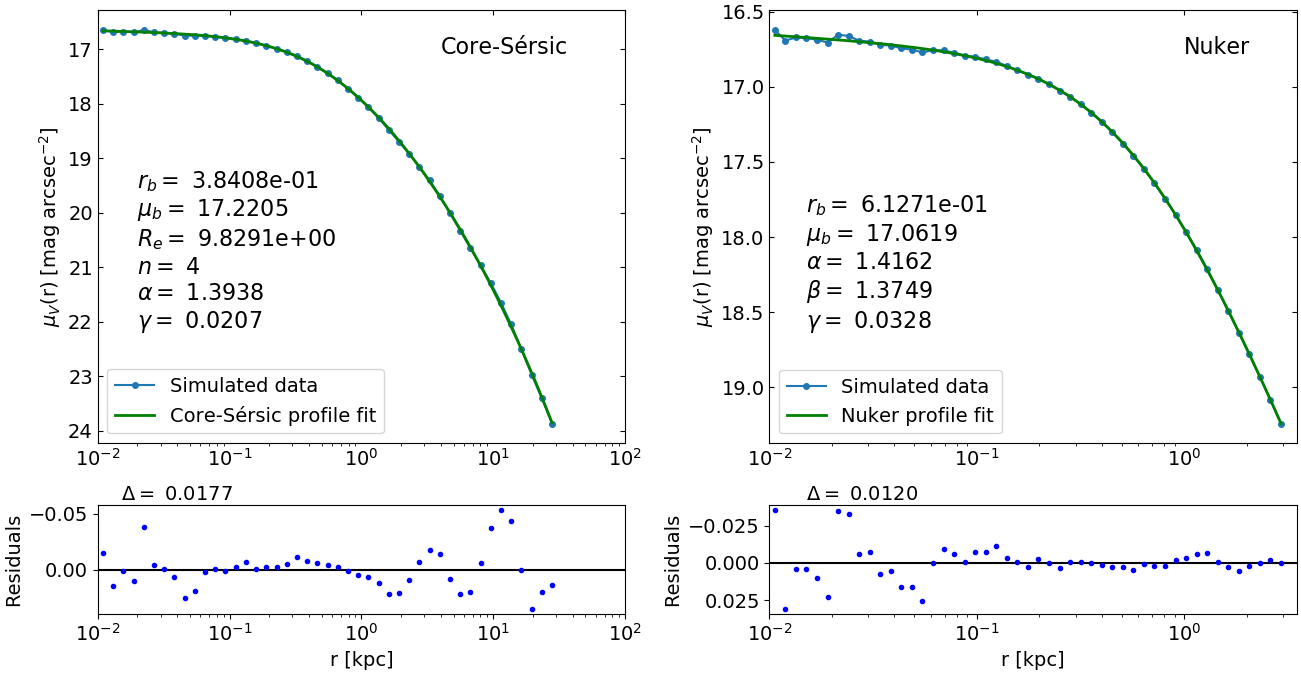
\includegraphics[width=\textwidth]{core_nuker_fits.png}
	\caption{Core-Sérsic and Nuker profile fits of surface brightness profiles calculated from Snapshot 3 (top-left and top-right figures). The best fit parameters are written on the figures, and are in the same units as the axes (i.e. $r_b$ and $R_e$ in kilo-parsecs, and $\mu_b$ in V-band magnitudes per arc-second squared). The relative residuals of the fits are plotted under their respective figures. The delta describes the root-mean-square of the residuals.}
	\label{figure:core_nuker}
\end{figure}

We use the "Levenberg-Marquardt" algorithm to fit core-Sérsic and Nuker models to surface brightness profiles that we have calculated. Figure \ref{figure:core_nuker} shows a comparison of the resulting fits for snapshot 3 (refer to table \ref{table:runs_and_snaps}), while figures \ref{figure:all_core} and \ref{figure:all_nuker}, located in the appendix, show the fits for every snapshot containing SMBH binaries. The values of the best-fit parameters are written on the figures, and looking at them, it is clear that the exact value of the best-fit break radius, i.e. the core radius estimate, depends quite heavily on the model used.

Which model is better for estimating the size of the core is up for debate \cite{Lauer2007, Dullo2012}. While the rms of the relative residuals seems to be consistently marginally smaller for the Nuker model when compared to the rms for the core-Sérsic model (compare figures \ref{figure:all_core} and \ref{figure:all_nuker}), one also has to take into account that in the Nuker model the best-fit value for $r_b$ is highly dependent on the fitting range \citep{Graham2003Nuker}. Furthermore, as stated by \cite{Rantala2018}, the fitting range of the Nuker model has to be narrowed down closer to the galactic core, in order to get sensible values for all of the model parameters ($\alpha \lesssim 1$ might prevent the model from describing the profile as a combination of two power-laws).

It is also possible to estimate the size of the core without model fitting by using the so-called "cusp radius" $r_\gamma$, which is the radius at which the negative logarithmic slope of the surface brightness density $\gamma'$ equals $1/2$ \citep{Carollo1997, Lauer2007Cusp}. The cusp radius $r_\gamma$ is also an estimation for the location where the inner power-law of the profile changes into the outer power-law, and thus equates to the core radius. 

We calculate $r_\gamma$ for all of the snapshots with SMBH binaries by calculating the first derivative (i.e. gradient) of the surface brightness profiles, and then using a "Nelder-Mead" minimization algorithm to find the radius, at which the gradient gets the value $-1/2$. 

Figure \ref{figure:radii_comparison} compares the core radius estimates from each of the three methods for every merger remnant from the snapshots. The break radii from the Nuker fits are consistently larger than the other core radius estimates, while also being the ones that, in general, agree least with the other values. However, a clear trend of, the size of the core growing with the masses of the central SMBHs of the merger progenitors, can be seen.

\begin{figure}[h]
	\centering
	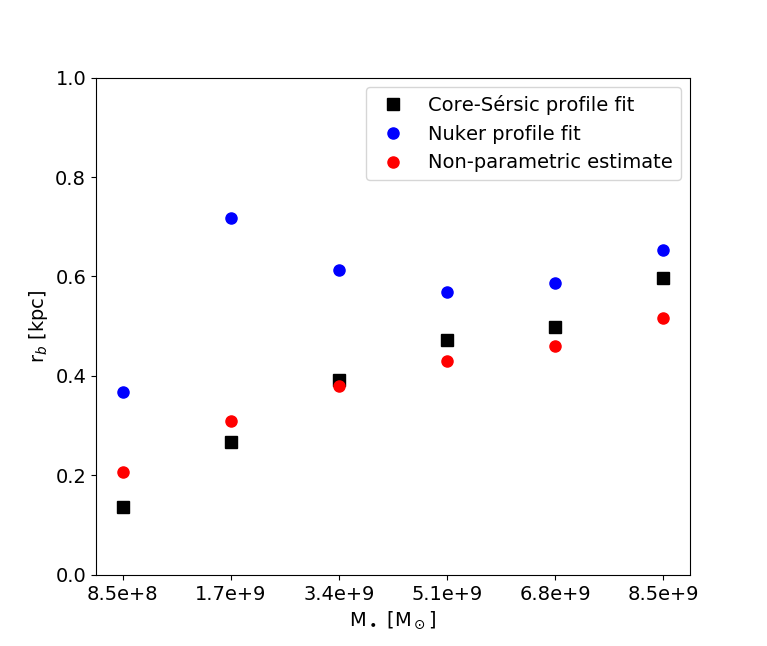
\includegraphics[width=0.7\textwidth]{rb_mass_relation.png}
	\caption{Comparison of core radii of the merger remnants, gained through three different methods: Core-Sérsic profile fitting (black squares), Nuker profile fitting (blue circles) and  finding the "cusp radius" (red circles). The x-axis shows the masses of the central SMBHs of the merger progenitors.}
	\label{figure:radii_comparison}
\end{figure}

\section{Velocity Anisotropy}

%\begin{figure}[h]
%	\centering
%	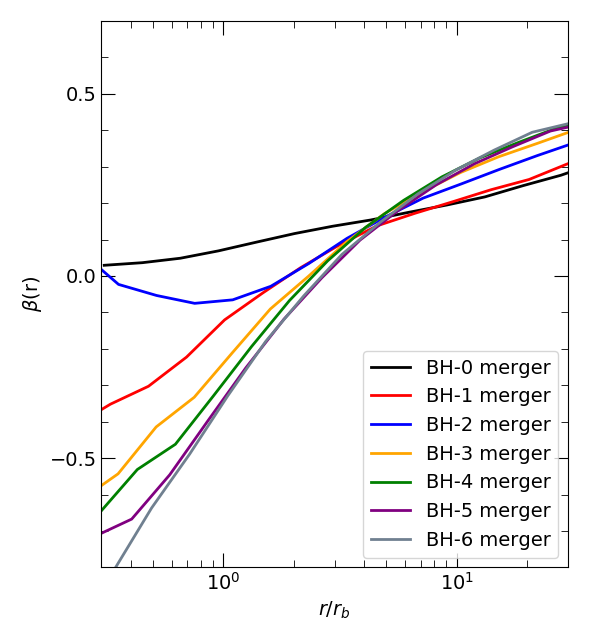
\includegraphics[width=0.9\textwidth]{beta.png}
%	\caption{Velocity anisotropy (beta) profiles of the simulated merger remnants with central black holes.}
%\end{figure}

One way of adding to the evidence that a galaxy has experienced core scouring by binary black holes, is to study its velocity anisotropy profile defined in \cite{BinneyTremaine}:
\begin{equation}
\beta(r) = 1 - \frac{\sigma_\theta^2 - \sigma_\phi^2}{2\sigma_r^2} = 1 - \frac{\sigma_t^2}{\sigma_r^2}, \label{eq:beta}
\end{equation}
where $\sigma_\theta$, $\sigma_\phi$ and $\sigma_r$ are velocity dispersions in the spherical coordinates, and $\sigma_t = \sqrt{(\sigma_\theta^2 + \sigma_\phi^2) / 2}$ is the tangential velocity dispersion. The $\beta$ parameter describes the relation between objects in radial and tangential orbits around the black hole binary, where a negative $\beta$ shows an abundance of tangential orbits, and positive an abundance of radial orbits. 

As the merging of two galaxies would cause a randomization of the stellar orbits, an area with negative $\beta$ (largely tangential stellar orbits) in the merger remnant, would imply that the stars on radial orbits have been ejected from the system. It has been shown that hardening black hole binaries can eject stars on highly radial orbits from the galactic core, which then causes the outer orbits to become more radial \citep{Quinlan1997, Milosavljevic2001, Thomas2014}, and looking at figure \ref{figure:beta_no_rb}, it seems like the same has happened in the simulations.

\begin{figure}[h]
	\centering
	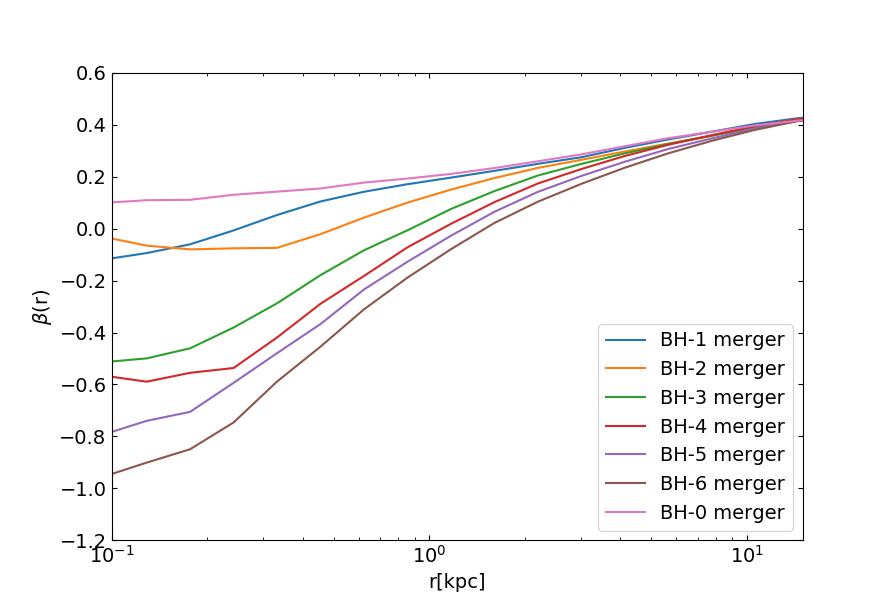
\includegraphics[width=0.9\textwidth]{beta_no_rb.png}
	\caption{Velocity anisotropy (beta) profiles of the simulated merger remnants with central black holes.}
	\label{figure:beta_no_rb}
\end{figure}

Figure \ref{figure:beta_no_rb} shows $\beta$-profiles calculated from the merger remnant simulation snapshots using equation \ref{eq:beta}. According to the profiles, the outer areas of the remnants are dominated by radial orbits, while the orbits near the centre are more tangential.




\section{Line-of-Sight Kinematics}

\section{Comparison to Observations}

\begin{figure}[h]
	\centering
	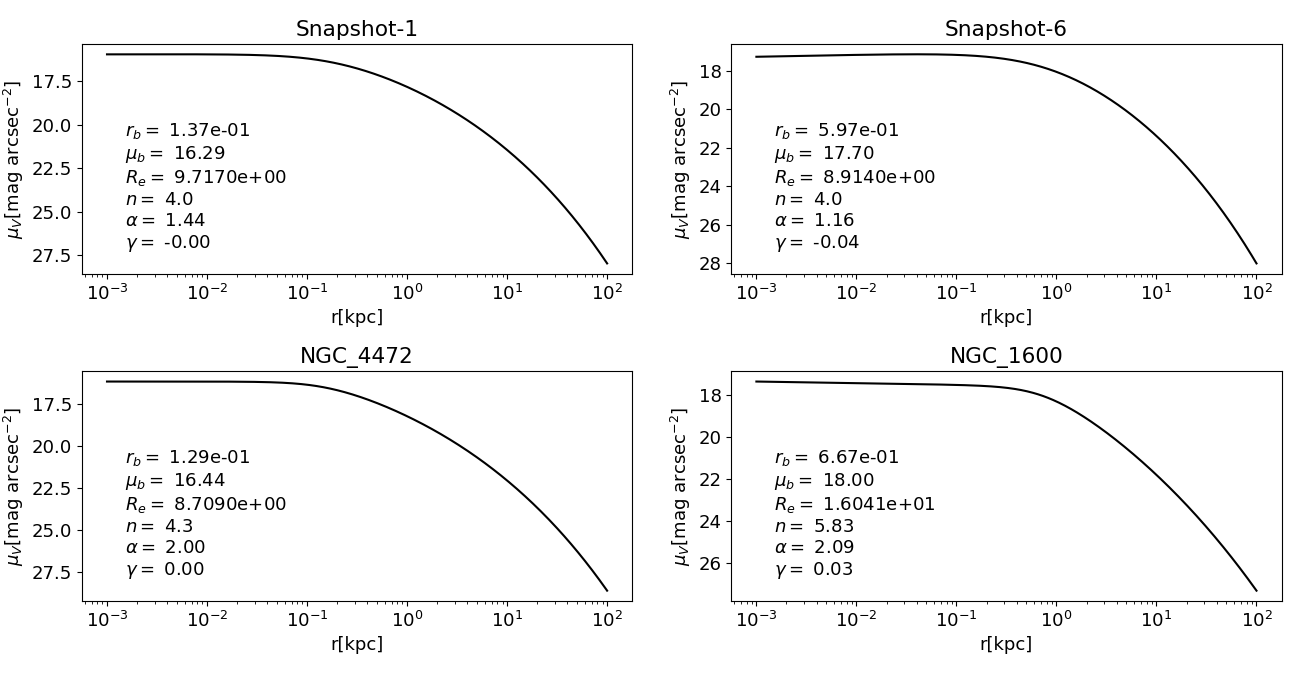
\includegraphics[width=\textwidth]{core_sersic_fits_obs_and_sim.png}
	\caption{Core-Sérsic profile fits of surface brightness profiles calculated from either merger simulation results (top figures) or observed galaxies (bottom figures). The respective fit parameters are written on the figures in units that correspond to the axes. The progenitors of the top-left simulation contained $8.5 \times 10^8 M_\odot$ mass central SMBHs, and $8.5 \times 10^9 M_\odot$ mass central SMBHs in the top-right simulation. The parameters for NGC1600's profile (bottom right), are changed from the units used by \cite{Thomas2016} to the above by assuming $V - R = 0.5$ (the same assumption being done by \cite{Lauer2007}), and by using the distance $D = 64 \mathrm{Mpc}$ \citep{Thomas2016} in order to define the relation between arc seconds and parsecs. As one can see, the profiles gained from simulations and observations are quite similar to each other.}
\end{figure}

\begin{figure}[h]
	\centering
	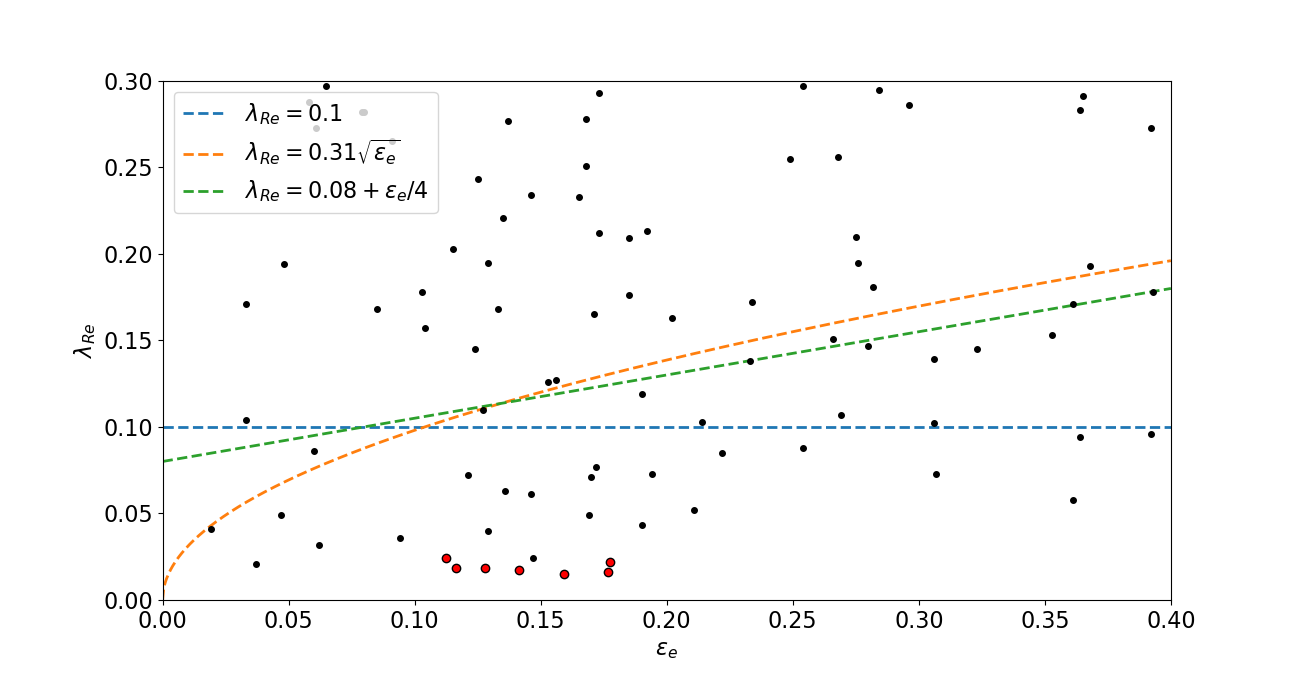
\includegraphics[width=\textwidth]{lambda_epsilon.png}
	\caption{The values of the $\lambda_{\mathrm{Re}}$-parameter of galaxies, plotted against their ellipticity at the effective radius. The red dots correspond to the simulated merger remnants, where as the black dots correspond to galaxies observed in the $\mathrm{ATLAS^{3D}}$-survey \citep{Emsellem2011}. The dashed lines display different slow rotator thresholds as a function of ellipticity.}
\end{figure}

\begin{figure}
	\centering
	\begin{subfigure}[b]{0.49\textwidth}
		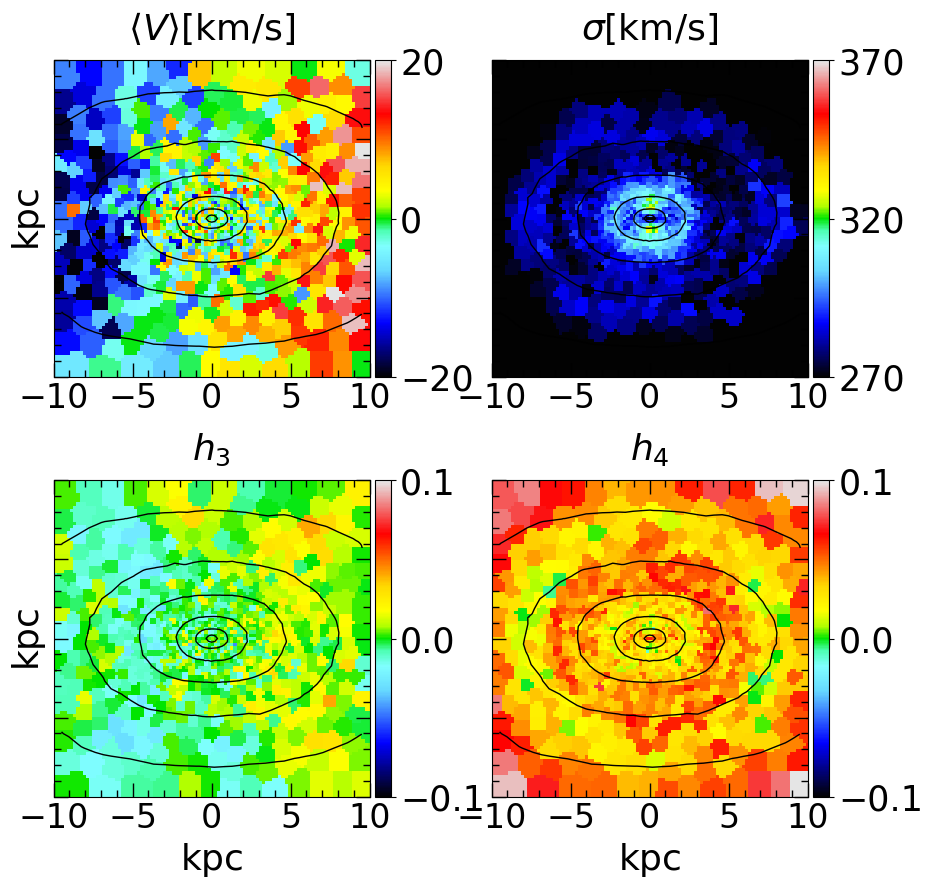
\includegraphics[width=\textwidth]{BH_0.png}
		\caption{BH-0}
	\end{subfigure}
	\begin{subfigure}[b]{0.49\textwidth}
		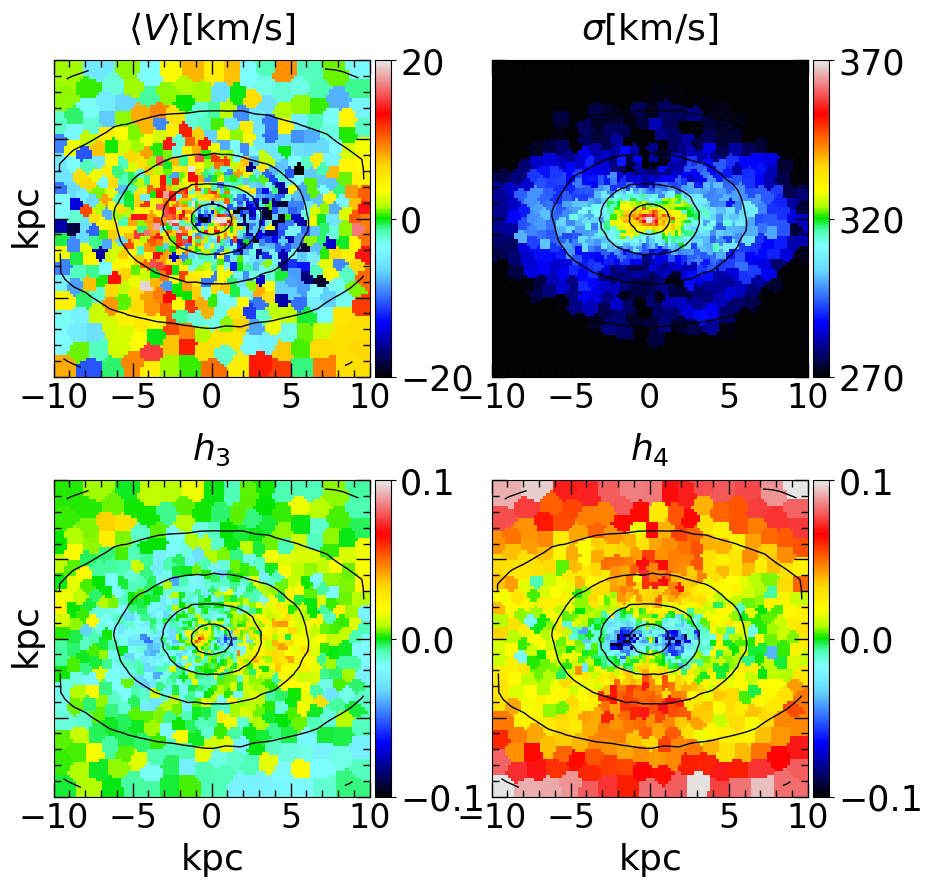
\includegraphics[width=\textwidth]{BH_6.png}
		\caption{BH-6}
	\end{subfigure}
	\caption{IFU-maps of average LOS-velocities, velocity dispersion, $h_3$ parameters and $h_4$ parameters from two simulated merger remnants. The four maps on the left are from a merger simulation where the progenitor galaxies had no central SMBHs, where as the four on the right are from a simulation with progenitor galaxies containing $M_\bullet = 8.5 \times 10^9 M_\odot$ central black holes.}
\end{figure}

\begin{figure}
	\centering
	\begin{subfigure}[b]{0.49\textwidth}
		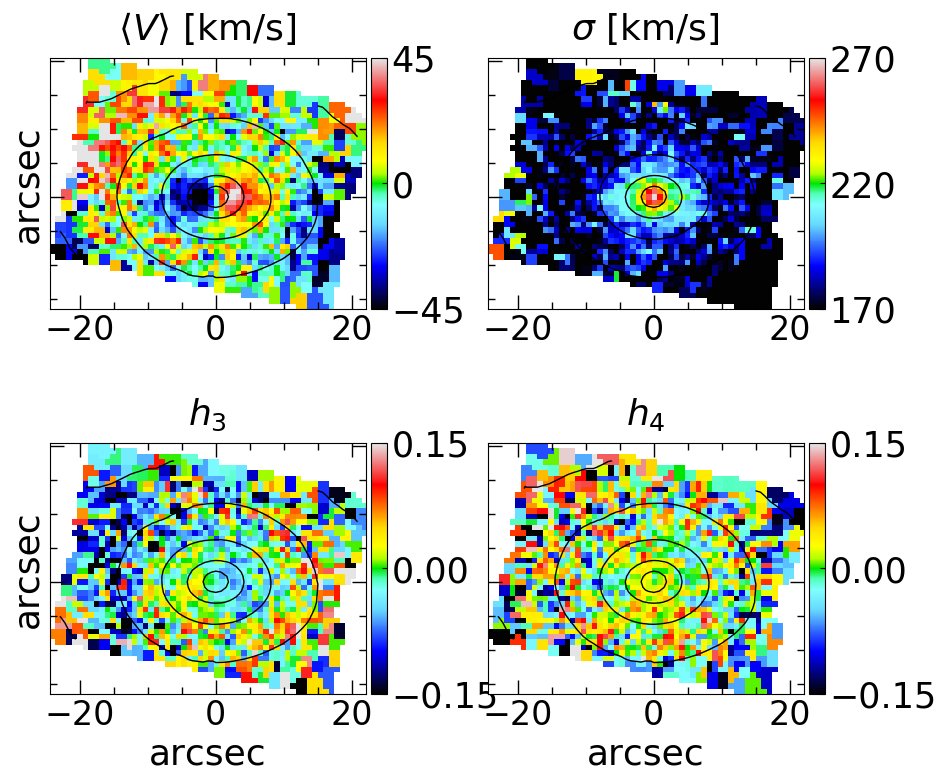
\includegraphics[width=\textwidth]{NGC3414_r6_voronoi.png}
		\caption{NGC 3414}
	\end{subfigure}
	\begin{subfigure}[b]{0.49\textwidth}
		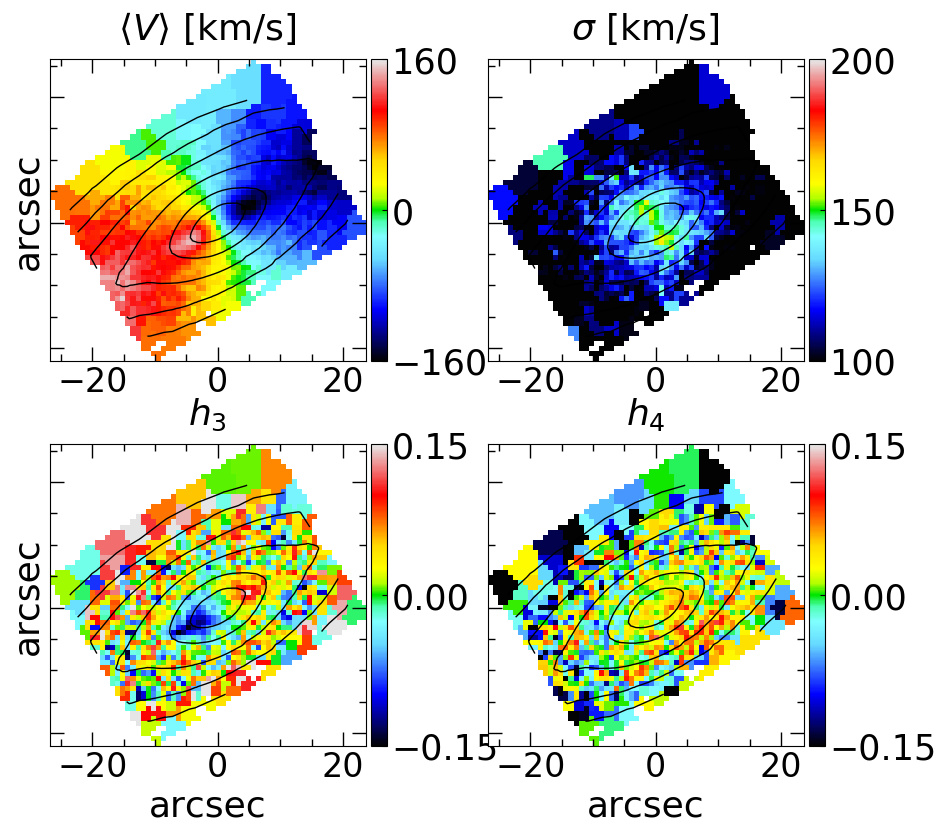
\includegraphics[width=\textwidth]{NGC4111_r1_voronoi.png}
		\caption{NGC 4111}
	\end{subfigure}
	\caption{IFU-maps of average LOS-velocities, velocity dispersion, $h_3$ parameters and $h_4$ parameters from ATLAS3D observations of two galaxies (NGC 3414 \citep{Emsellem2004} and NGC 4111 \citep{Cappellari2011}).}
\end{figure}

\begin{table}
	\begin{center}
		\scriptsize
		\begin{tabular}{c c c c c c c c c c}
		\hline
		\hline
		Galaxy & $M_\star$ & $M_\bullet$ & $R_e$ & $\mu_e$ & $n$ & 
		$\langle V_\mathrm{LOS} \rangle$ & $\sigma_e$ & $\lambda_e$ &
		$\epsilon_e$ \\
		& $[\times 10^{11} M_\odot]$ & $[\times 10^{10} M_\odot]$ &
		[kpc] & [$\mathrm{mag/arcsec^2}$] & & [km/s] & [km/s] & & \\
		(1) & (2) & (3) & (4) & (5) & (6) & (7) & (8) & (9) & (10) \\
		\hline
		BH-6 & $4.960$ & $2 \times 0.85$ & $5.507$ & $20.26$ & $4$ & $6.9$ & $311$ & $0.024$ & $0.11$ \\
		NGC 1600 & $5.0$ & $1.7$ & $\sim 16$ & $(22.53)$ & $5.83$ & $3.4$ & 
		$293$ & $0.026$ & $032$ \\
		\hline
		\end{tabular}
	\end{center}
	\caption{Comparison between the physical properties of the simulated merger remnant "BH-6" and the galaxy NGC 1600. The properties described in the columns of the table are explained below, with the sources for the properties of NGC 1600 being written inside the brackets. \\
	(1) Name of the galaxy. \\
	(2) Total stellar mass \citep{Thomas2016}. \\
	(3) Central black hole mass \citep{Thomas2016}. \\
	(4) Effective radius \citep{Thomas2016}. For NGC 1600, the effective radius is changed from arc seconds to kpc by assuming that it is located at the distance of $D = 64 \; \mathrm{Mpc}$ \citep{Thomas2016}. \\
	(5) Surface brightness at the effective radius. \\
	(6) Sérsic index from the best fitting core-Sérsic profile fit \citep{Thomas2016}. \\
	(7) Mean line-of-sight velocity inside the effective radius \citep{Bender1994}. \\
	(8) Velocity dispersion inside the effective radius \citep{Veale2017veldisp}. For "BH-6", the given velocity dispersion is calculated from a Voronoi binned image as the mean of the velocity dispersion values of the bins located inside the effective radius. \\
	(9) Spin parameter at the effective radius \citep{Veale2018lambda}. \\
	(10) For "BH-6": ellipticity of the galaxy at the effective radius; and for GC 1600: luminosity weighted ellipticity \citep{Goullaud2018}.
	}
\end{table}


\section{Implications}


\chapter{Conclusions}

\appendix

\chapter{Figures}

\begin{figure}
	\centering
	\begin{subfigure}[b]{0.49\textwidth}
		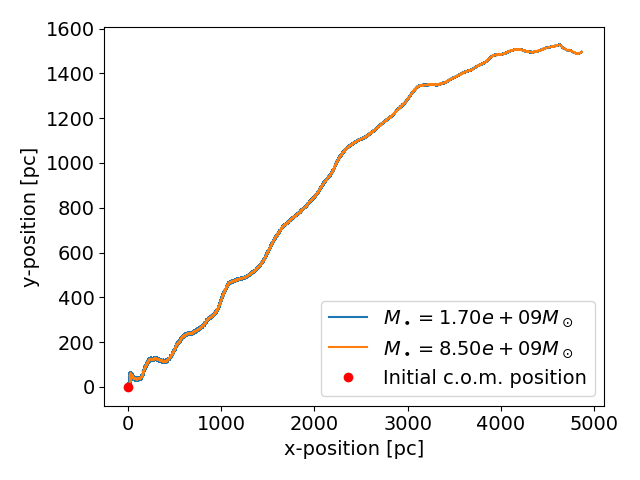
\includegraphics[width=\textwidth]{Run1_Trajectory_small.png}
		\caption{Run 1}
	\end{subfigure}
	\begin{subfigure}[b]{0.49\textwidth}
		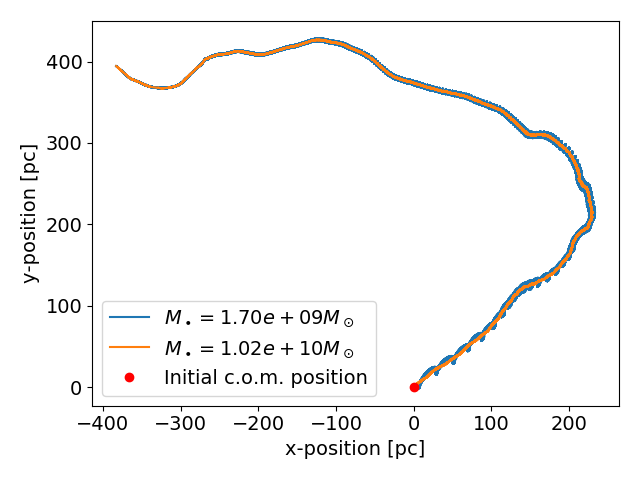
\includegraphics[width=\textwidth]{Run2_Trajectory_small.png}
		\caption{Run 2}
	\end{subfigure}
	\begin{subfigure}[b]{0.49\textwidth}
		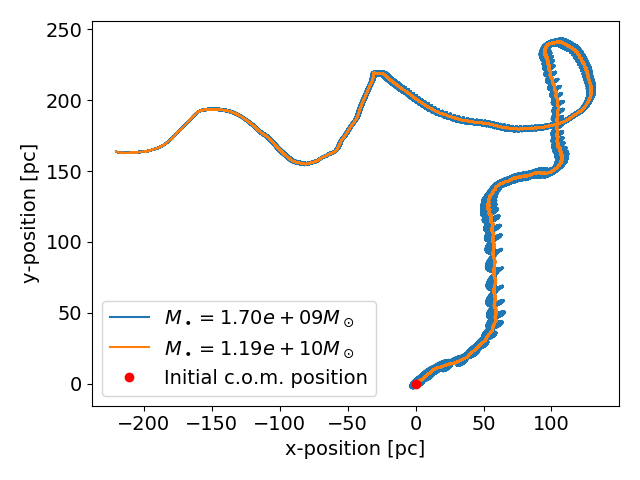
\includegraphics[width=\textwidth]{Run3_Trajectory_small.png}
		\caption{Run 3}
	\end{subfigure}
	\begin{subfigure}[b]{0.49\textwidth}
		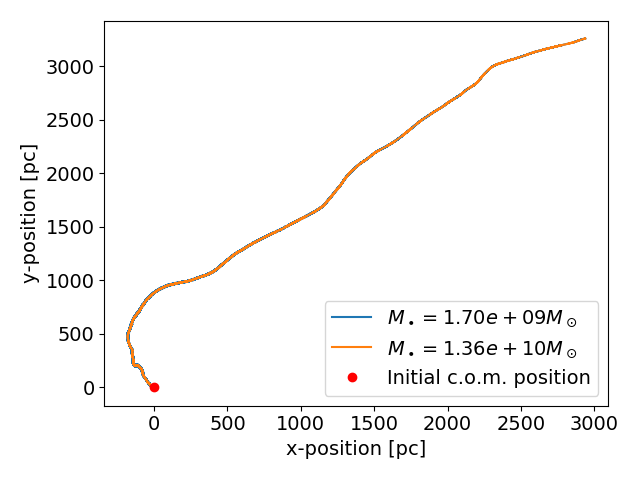
\includegraphics[width=\textwidth]{Run4_Trajectory_small.png}
		\caption{Run 4}
	\end{subfigure}
	\caption{The trajectories of the black holes from simulation runs by \cite{Mannerkoski2019}. The coordinates are centred on the initial location of the centre-of-mass of the black hole system. The orange and blue lines show the paths taken by the smaller and larger black holes respectively during the simulation.}
\end{figure}

\begin{figure}[h]
	\centering
	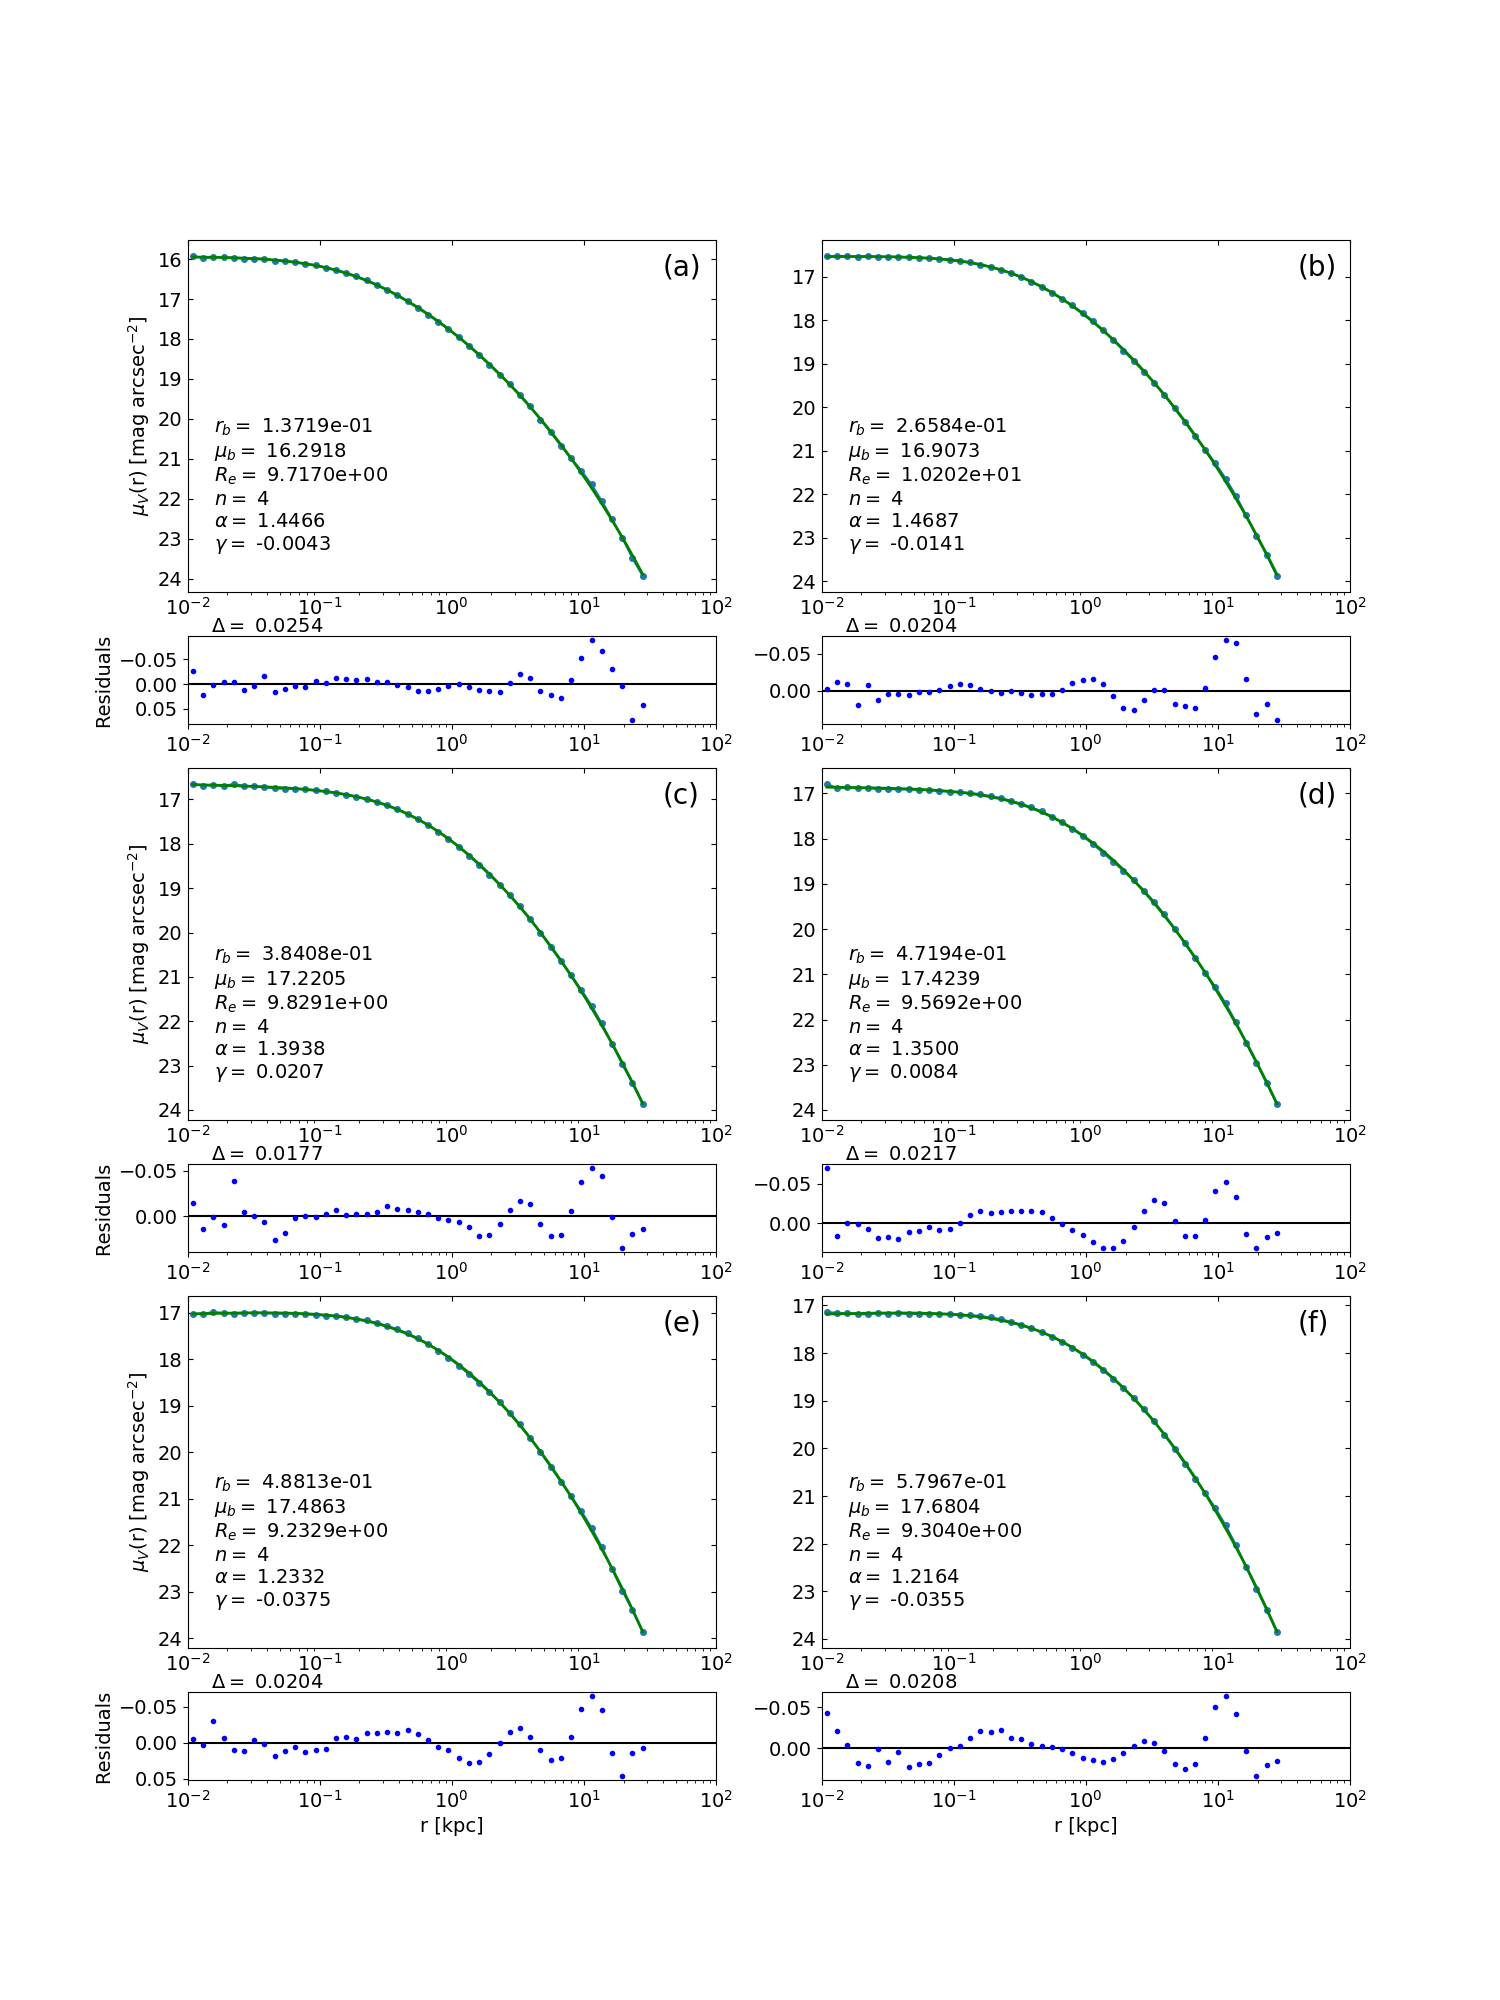
\includegraphics[width=\textwidth]{all_core_profiles.png}
	\caption{Core-Sérsic profile fits of the surface brightness data calculated from all of the individual simulated merger remnants with progenitors containing central supermassive black holes. The letters (a)-(f) denote the different snapshots ((a): BH-1, (b): BH-2, (c): BH-3, (d): BH-4, (e): BH-5, (f): BH-6).}
	\label{figure:all_core}
\end{figure}

\begin{figure}[h]
	\centering
	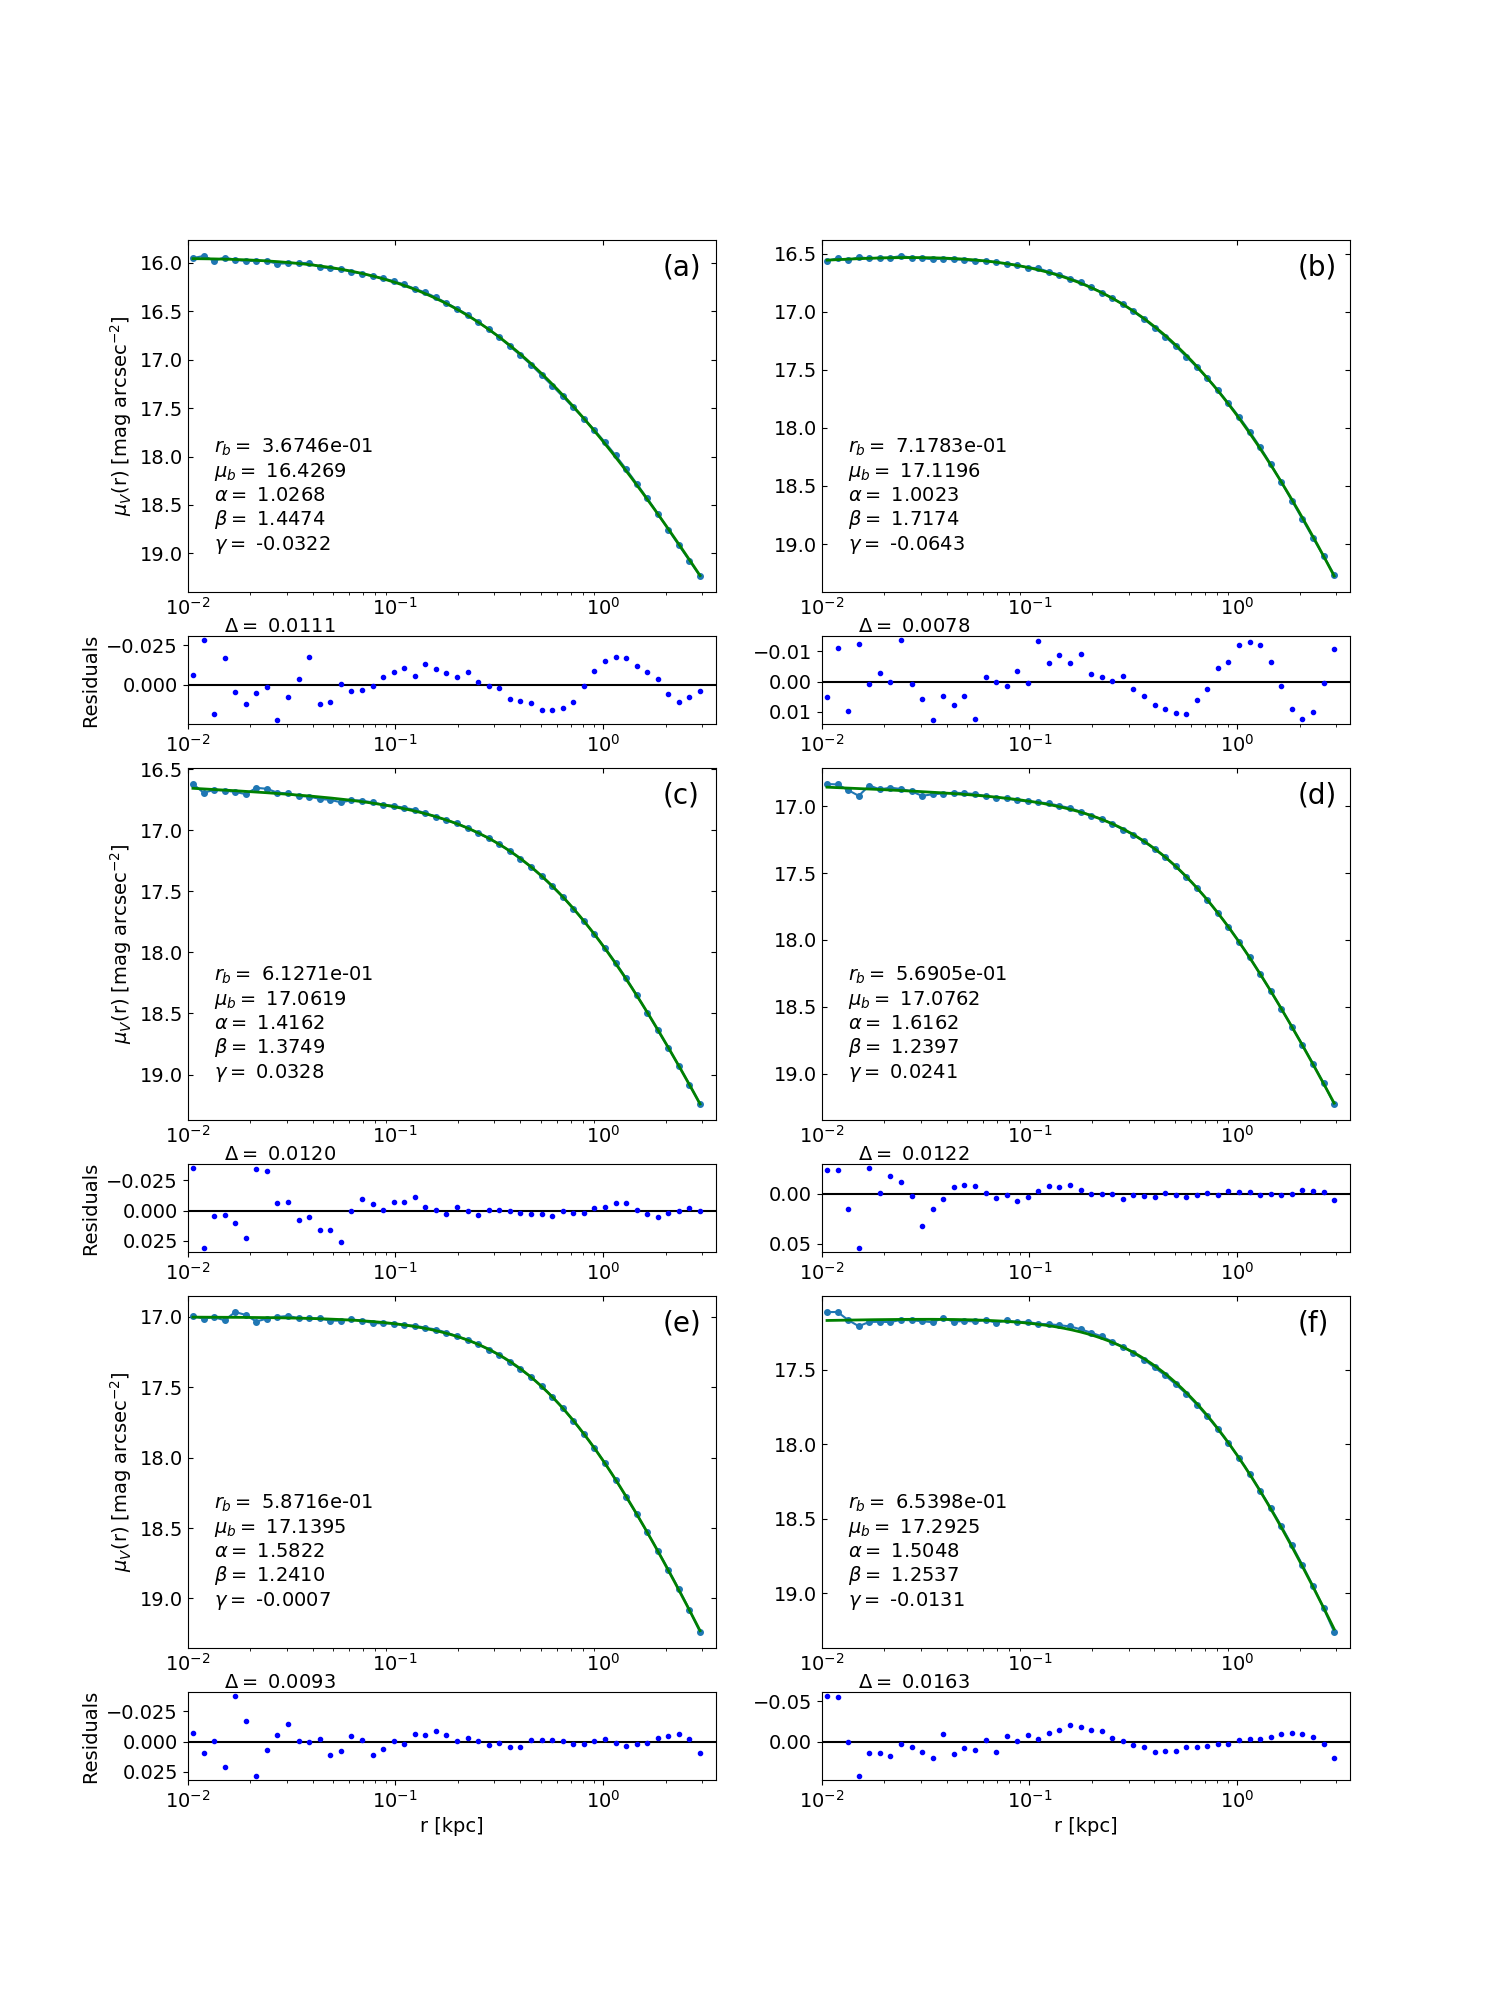
\includegraphics[width=\textwidth]{all_nuker_profiles.png}
	\caption{Nuker profile fits of the surface brightness data calculated from all of the individual simulated merger remnants with progenitors containing central supermassive black holes. The letters (a)-(f) denote the different merger remnants ((a): BH-1, (b): BH-2, (c): BH-3, (d): BH-4, (e): BH-5, (f): BH-6).}
	\label{figure:all_nuker}
\end{figure}

\begin{figure}
	\centering
	\begin{subfigure}[b]{0.49\textwidth}
		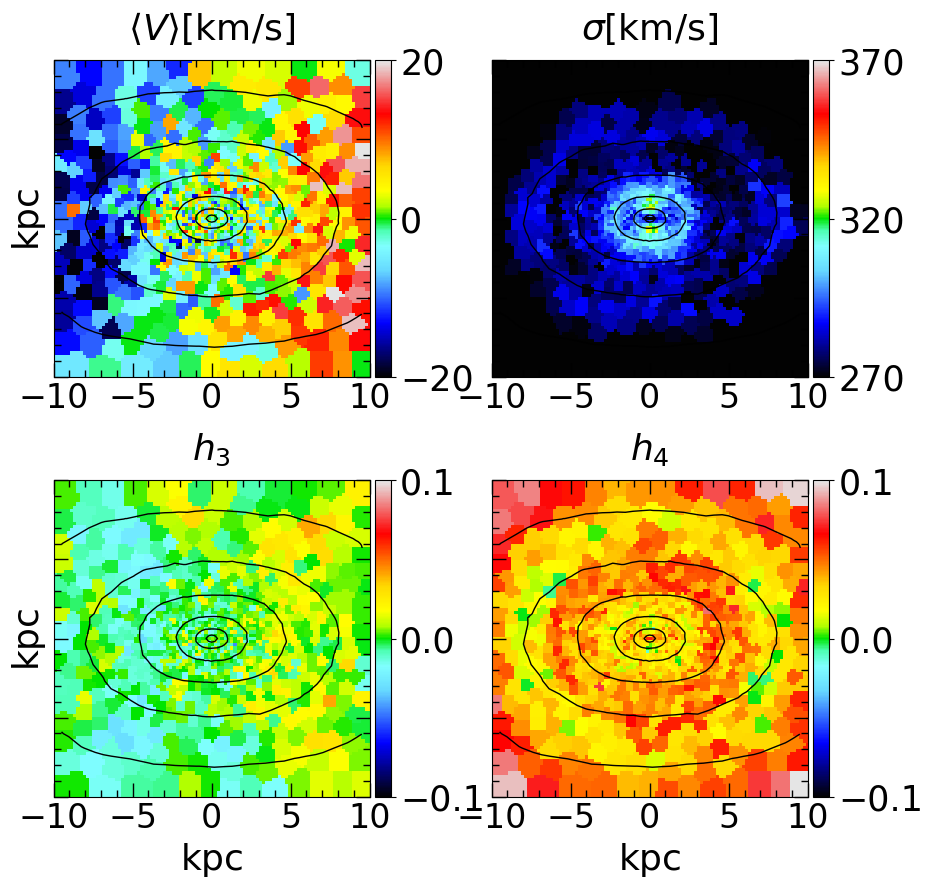
\includegraphics[width=\textwidth]{BH_0.png}
		\caption{BH-0}
	\end{subfigure}
	\begin{subfigure}[b]{0.49\textwidth}
		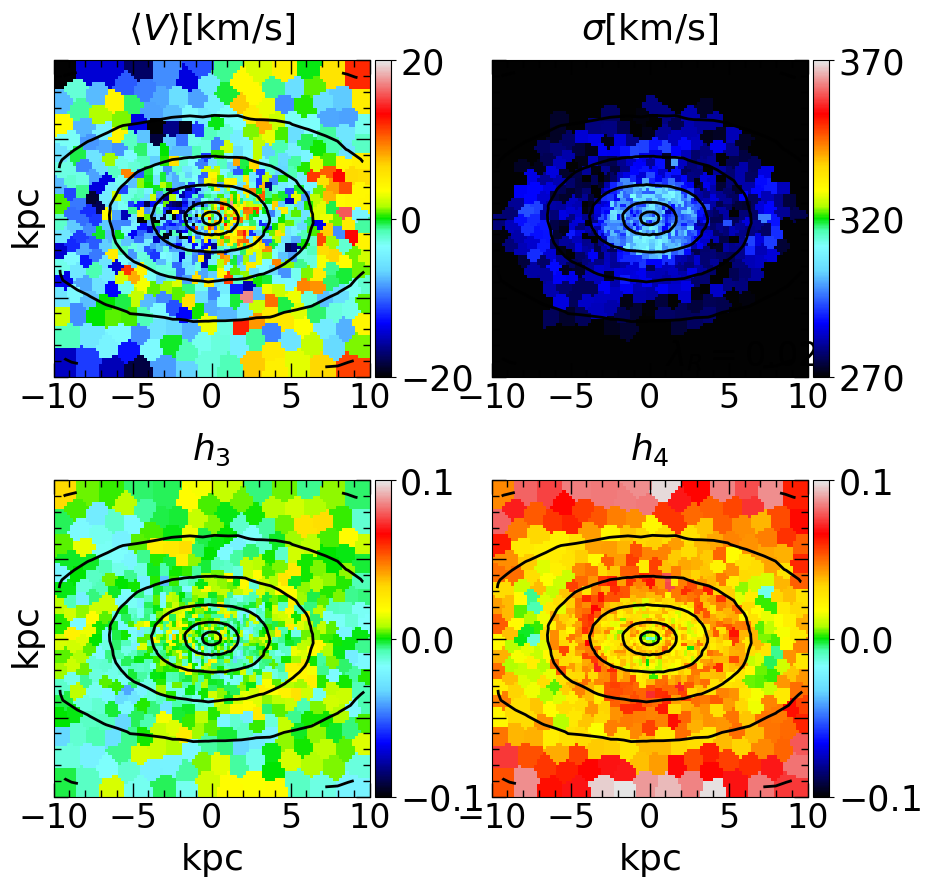
\includegraphics[width=\textwidth]{BH_1.png}
		\caption{BH-1}
	\end{subfigure}
	\begin{subfigure}[b]{0.49\textwidth}
		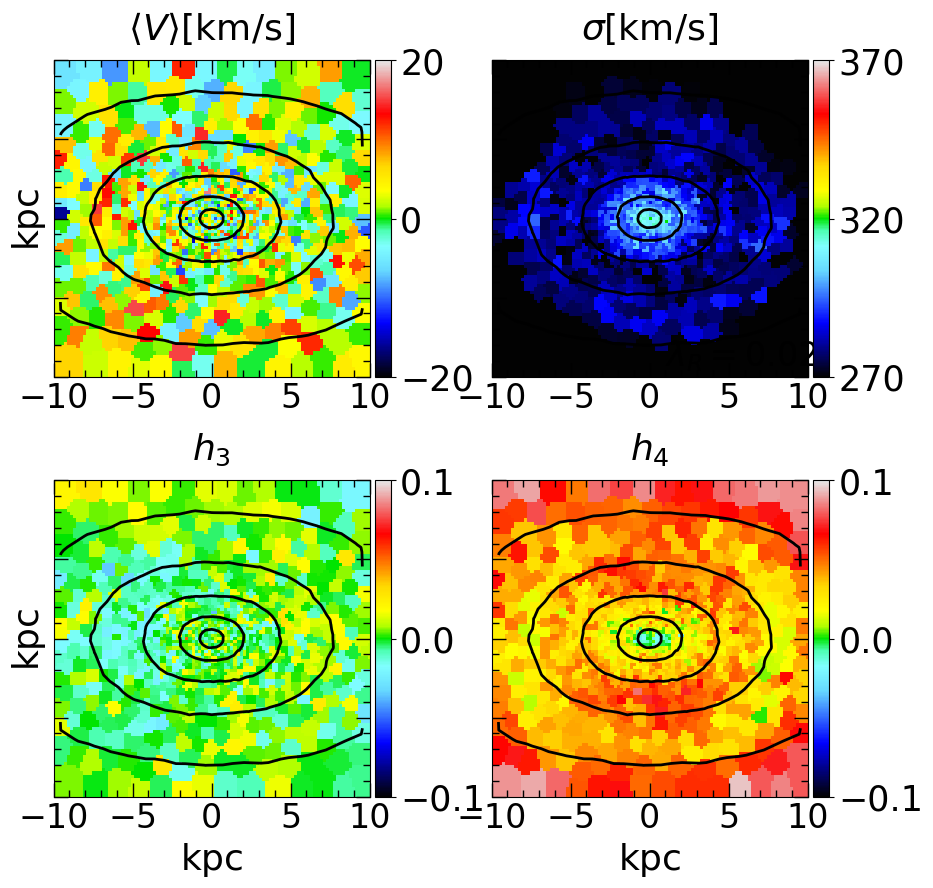
\includegraphics[width=\textwidth]{BH_2.png}
		\caption{BH-2}
	\end{subfigure}
	\begin{subfigure}[b]{0.49\textwidth}
		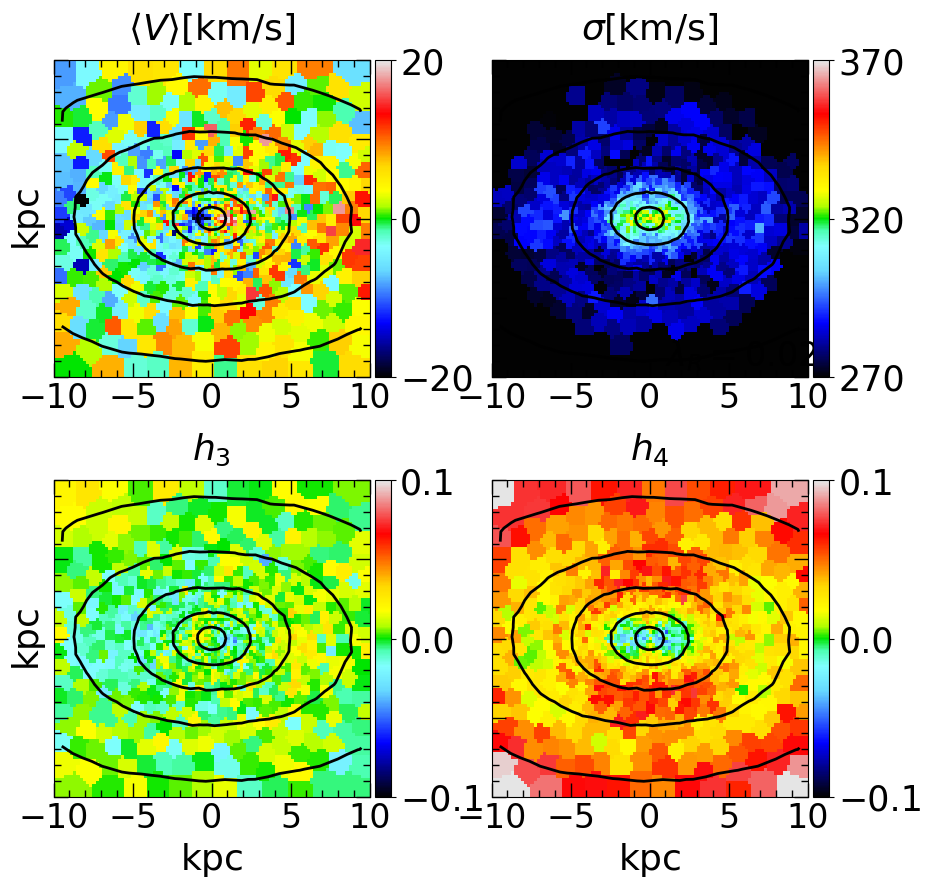
\includegraphics[width=\textwidth]{BH_3.png}
		\caption{BH-3}
	\end{subfigure}
	\caption{IFU-maps of average LOS-velocities, velocity dispersion, $h_3$ parameters and $h_4$ parameters from four simulated merger remnants: BH-0, BH-1, BH-2 and BH-3.}
\end{figure}

\begin{figure}
	\centering
	\begin{subfigure}[b]{0.49\textwidth}
		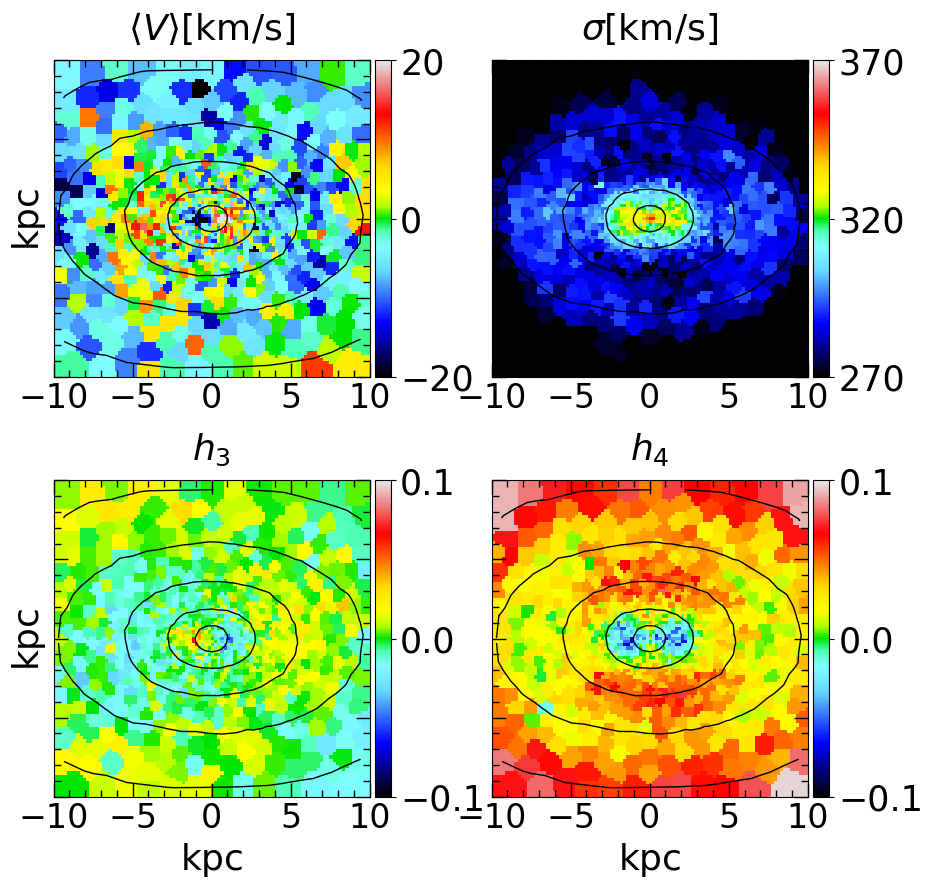
\includegraphics[width=\textwidth]{BH_4.png}
		\caption{BH-4}
	\end{subfigure}
	\begin{subfigure}[b]{0.49\textwidth}
		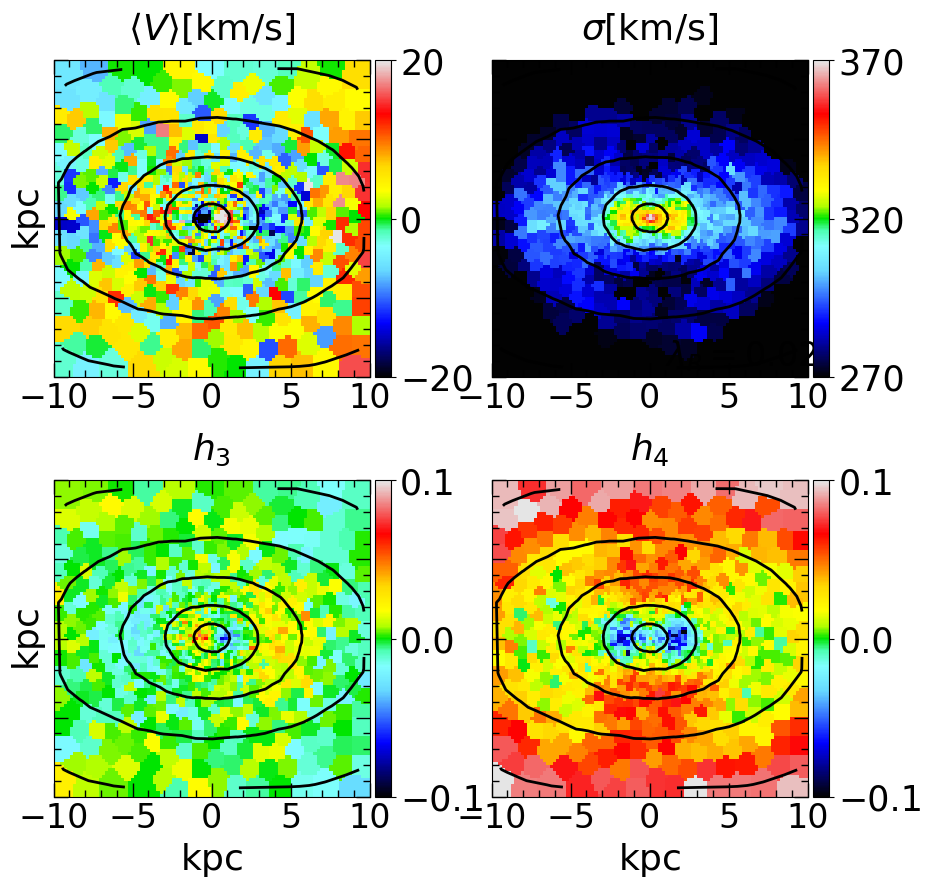
\includegraphics[width=\textwidth]{BH_5.png}
		\caption{BH-5}
	\end{subfigure}
	\begin{subfigure}[b]{0.49\textwidth}
		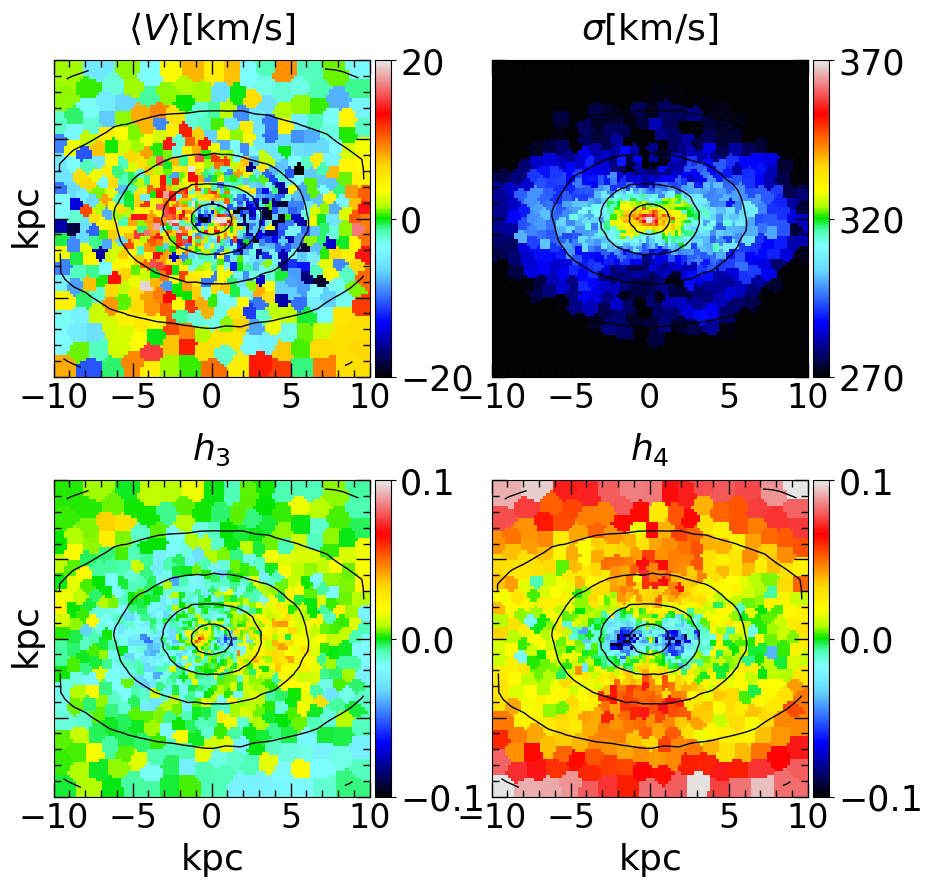
\includegraphics[width=\textwidth]{BH_6.png}
		\caption{BH-6}
	\end{subfigure}
	\caption{IFU-maps of average LOS-velocities, velocity dispersion, $h_3$ parameters and $h_4$ parameters from three simulated merger remnants: BH-4, BH-5 and BH-6.}
\end{figure}

% STEP 5:
% Uncomment the following lines and set your .bib file and desired bibliography style
% to make a bibliography with BibTeX.
% Alternatively you can use the thebibliography environment if you want to add all
% references by hand.


% Define journal names
\newcommand{\apj}{The Astrophysical Journal}
\newcommand{\mnras}{Monthly Notices of the Royal Astronomical Society}
\newcommand{\apjs}{The Astrophysical Journal Supplement}
\newcommand{\nat}{Nature}
\newcommand{\aj}{The Astronomical Journal}
\newcommand{\na}{New Astronomy}

\clearpage
\addcontentsline{toc}{chapter}{Bibliography} % This lines adds the bibliography to the ToC
\bibliographystyle{plainnat}
\bibliography{bibliography.bib}


\end{document}

